%-------------------------------------------------------------------------------
%-------------------------------------------------------------------------------
\chapter{Présentation}
%-------------------------------------------------------------------------------
%-------------------------------------------------------------------------------
\thispagestyle{empty}
%-------------------------------------------------------------------------------
%-------------------------------------------------------------------------------
\section{Qu'est-ce que l'informatique ?}
%-------------------------------------------------------------------------------
La Société Informatique de France (SIF) propose la définition suivante.
%-------------------------------------------------------------------------------
\begin{defin}[informatique]
L'informatique est la science et la technique de la représentation de l'information d'origine artificielle ou naturelle, ainsi que des processus algorithmiques de collecte, stockage, analyse, transformation et communication de cette information, exprimés dans des langages formels ou des langues naturelles et effectués par des machines ou des êtres humains, seuls ou collectivement.
\end{defin}
%-------------------------------------------------------------------------------
Cette définition, très structurée, mérite des éclaircissements.
%-------------------------------------------------------------------------------
\begin{description}
\item[Information] 
L'informatique à pour objet l'information. 
Cela peut sembler une évidence quand on regarde l'étymologie mais le nom anglais, {\bf computer science}, ne le laissait pas deviner.

Lorsque plusieurs processus ou agents interagissent dans la poursuite d'un but commun ils doivent échanger de l'information. L'informatique est ce qui permet ces échanges d'informations. 
%-------------------------------------------------------------------------------
\item[Machines]
L'informatique utilise des machines, les ordinateurs.

Mais l'informatique n'est pas {\bf que} la science des ordinateurs : de la même manière que l'astronomie n'est pas que la science des télescopes. Passés les premiers temps héroïques où les prouesses nouvelles des machines nous émerveillaient, l'informatique nous permet de comprendre ce que font les ordinateurs et ce qu'ils ne peuvent pas faire. L'informatique est ce qui rend possible l'existence et l'usage des ordinateurs.

Les ordinateurs sont des machines rapides et fiables : ils permettent d'automatiser des tâches fastidieuses et répétées. En ce sens on peut en voir l'origine dans les machines automatiques : les calculatrices mécaniques, le métier à tisser Jacquard, les orgues de Barbaries, \dots Mais une évolution remarquable est que les ordinateurs ne sont pas spécialisés dans un travail unique : ils sont programmables. La première tâche d'un ordinateur est de recevoir les instructions qu'il aura à exécuter.
%-------------------------------------------------------------------------------
\item[Langages]
 On a donc besoin d'un langage commun entre les humains et les machines : un langage informatique est le moyen de traduire nos instructions à une machine. Comme celle-ci manque cruellement d'imagination et d'anticipation nous sommes contraints de faire un travail de formalisation qui nous permet de décomposer en tâches simples le travail que nous souhaitons faire faire à l'ordinateur.
%-------------------------------------------------------------------------------
\item[Science et technique] 

L'informatique est une science : elle produit des énoncés qui seront évalués selon le critère de vérité.
%-------------------------------------------------------------------------------
La science informatique est née au début du vingtième siècle par les résultats de mathématiciens (Turing, Gödel, Curry, \dots) qui cherchaient à déterminer les calculs mathématiques qui sont {\bf effectivement} réalisables, c'est-à-dire représentables par un algorithme avec le vocabulaire actuel.

La science informatique ne peut être séparée de la question de la réalisation effective : elle cherche à savoir ce qui peut être fait et cherche à faire ce qui peut être fait.
%-------------------------------------------------------------------------------
\item[Autres sciences]
Comme son objet est l'information l'informatique est étroitement liée aux autres sciences.

Elle étudiera souvent les mêmes phénomènes que d'autres sciences mais {\it différemment}.

Un exemple  : les images. 

\begin{itemize}
\item Un physicien étudie   les images sous forme de propagation de rayons lumineux. Cela permet la construction de verres qui corrigent la vue ou de lentilles pour les appareils
photo.
\item Avec la photo argentique, la chimie permet la reproduction d'images sur une surface par dépôt de pigments colorés qui se fixent sur la surface.
\item Les géomètres mathématiciens s'intéressent aux formes qui constituent les images dans le plan ou dans l'espace (et généralisent ensuite dans des espaces plus généraux).
\item Les médecins soignent les problèmes de l'œil et des nerfs optiques qui nous permettent de voir les images.
\item L'informatique  appréhende  les images en les {\it pixélisant} elle en traduit l'information, ce qui permet de la transmettre, la reproduire, la compresser, la transformer, la caractériser \dots.
\end{itemize}

Les appareils photo numériques apparus il y a une vingtaine d’années sont le fruit des efforts conjoints de physiciens et d'informaticiens
\end{description}

\subsection{Qu'est-ce qu'un ordinateur ?}

C'est un truisme de dire aujourd'hui que les ordinateurs sont partout : des machines installées sur un bureau aux serveurs dans des salles climatisées, mais aussi dans les téléphones, les télévisions, les appareils photos, les liseuses, les voitures\dots{} et avec la généralisation des «objets connectés», on en trouve jusque dans les ampoules.

Tant et si bien que l'on peut ressentir une certaine confusion en tentant de préciser ce qu'est un ordinateur. On peut commencer par lister les éléments communs suivants :
	\begin{itemize}
	\item il reçoit des informations par l'intermédiaire d'un utilisateur ou d'un réseau ;
	\item il émet des informations via le réseau ou un de ses périphériques ;
	\item il a besoin d'une source d'énergie pour fonctionner.
	\end{itemize}
Néanmoins cette première tentative s'avère infructueuse, car il n'est pas difficile de trouver des contre-exemples : un scooter nécessite une source d'énergie, il reçoit des informations de la part de son conducteur, il en émet sous la forme de signaux lumineux indiquant le niveau d'huile, de carburant\dots{} mais ce n'est pas un ordinateur.

En fin de compte, ce qui caractérise un ordinateur est plutôt sa capacité à \emph{mener des calculs}. D'ailleurs, le terme \emph{computer} est lié en Anglais au verbe \emph{to compute} : calculer.

Nous allons partir d'un ordinateur tel qu'il se présente aujourd'hui sous sa forme la plus reconnaissable (un «ordinateur personnel») et survoler le rôle de chacun de ses composants, avant de plonger dans les détails et de revenir sur les interrogations ci-dessus. 
%-------------------------------------------------------------------------------
\newpage
%-------------------------------------------------------------------------------
%-------------------------------------------------------------------------------
\section{Soulevons le capot !}
%-------------------------------------------------------------------------------
%-------------------------------------------------------------------------------
%-------------------------------------------------------------------------------
\subsection{De multiples périphériques et composants}
%-------------------------------------------------------------------------------
%-------------------------------------------------------------------------------
Clavier, disque dur, clef USB, carte graphique\dots{} Tout le monde a entendu ces termes, mais n'est pas forcément au fait de la manière dont ils s'articulent et communiquent pour accomplir leur fonction.

Passons sur les «périphériques externes», que tout le monde connaît au moins de vue (figures~\ref{fig:apple-magic-keyboard-wireless} à~\ref{fig:hp_deskjet}). Leur fonction est en général plutôt intuitive (mais leur fonctionnement, lui, beaucoup moins !)
%-------------------------------------------------------------------------------
\begin{figure}[!htb]
\centering
	\begin{subfigure}[b]{0.3\textwidth}
	\centering
	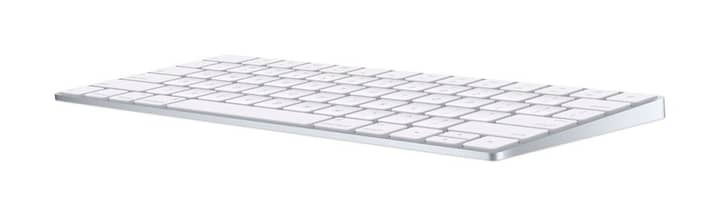
\includegraphics[width=5cm]{Machines/apple-magic-keyboard-wireless.jpg}
	\caption{\label{fig:apple-magic-keyboard-wireless}}
	\end{subfigure}
\quad
	\begin{subfigure}[b]{0.2\textwidth}
	\centering
	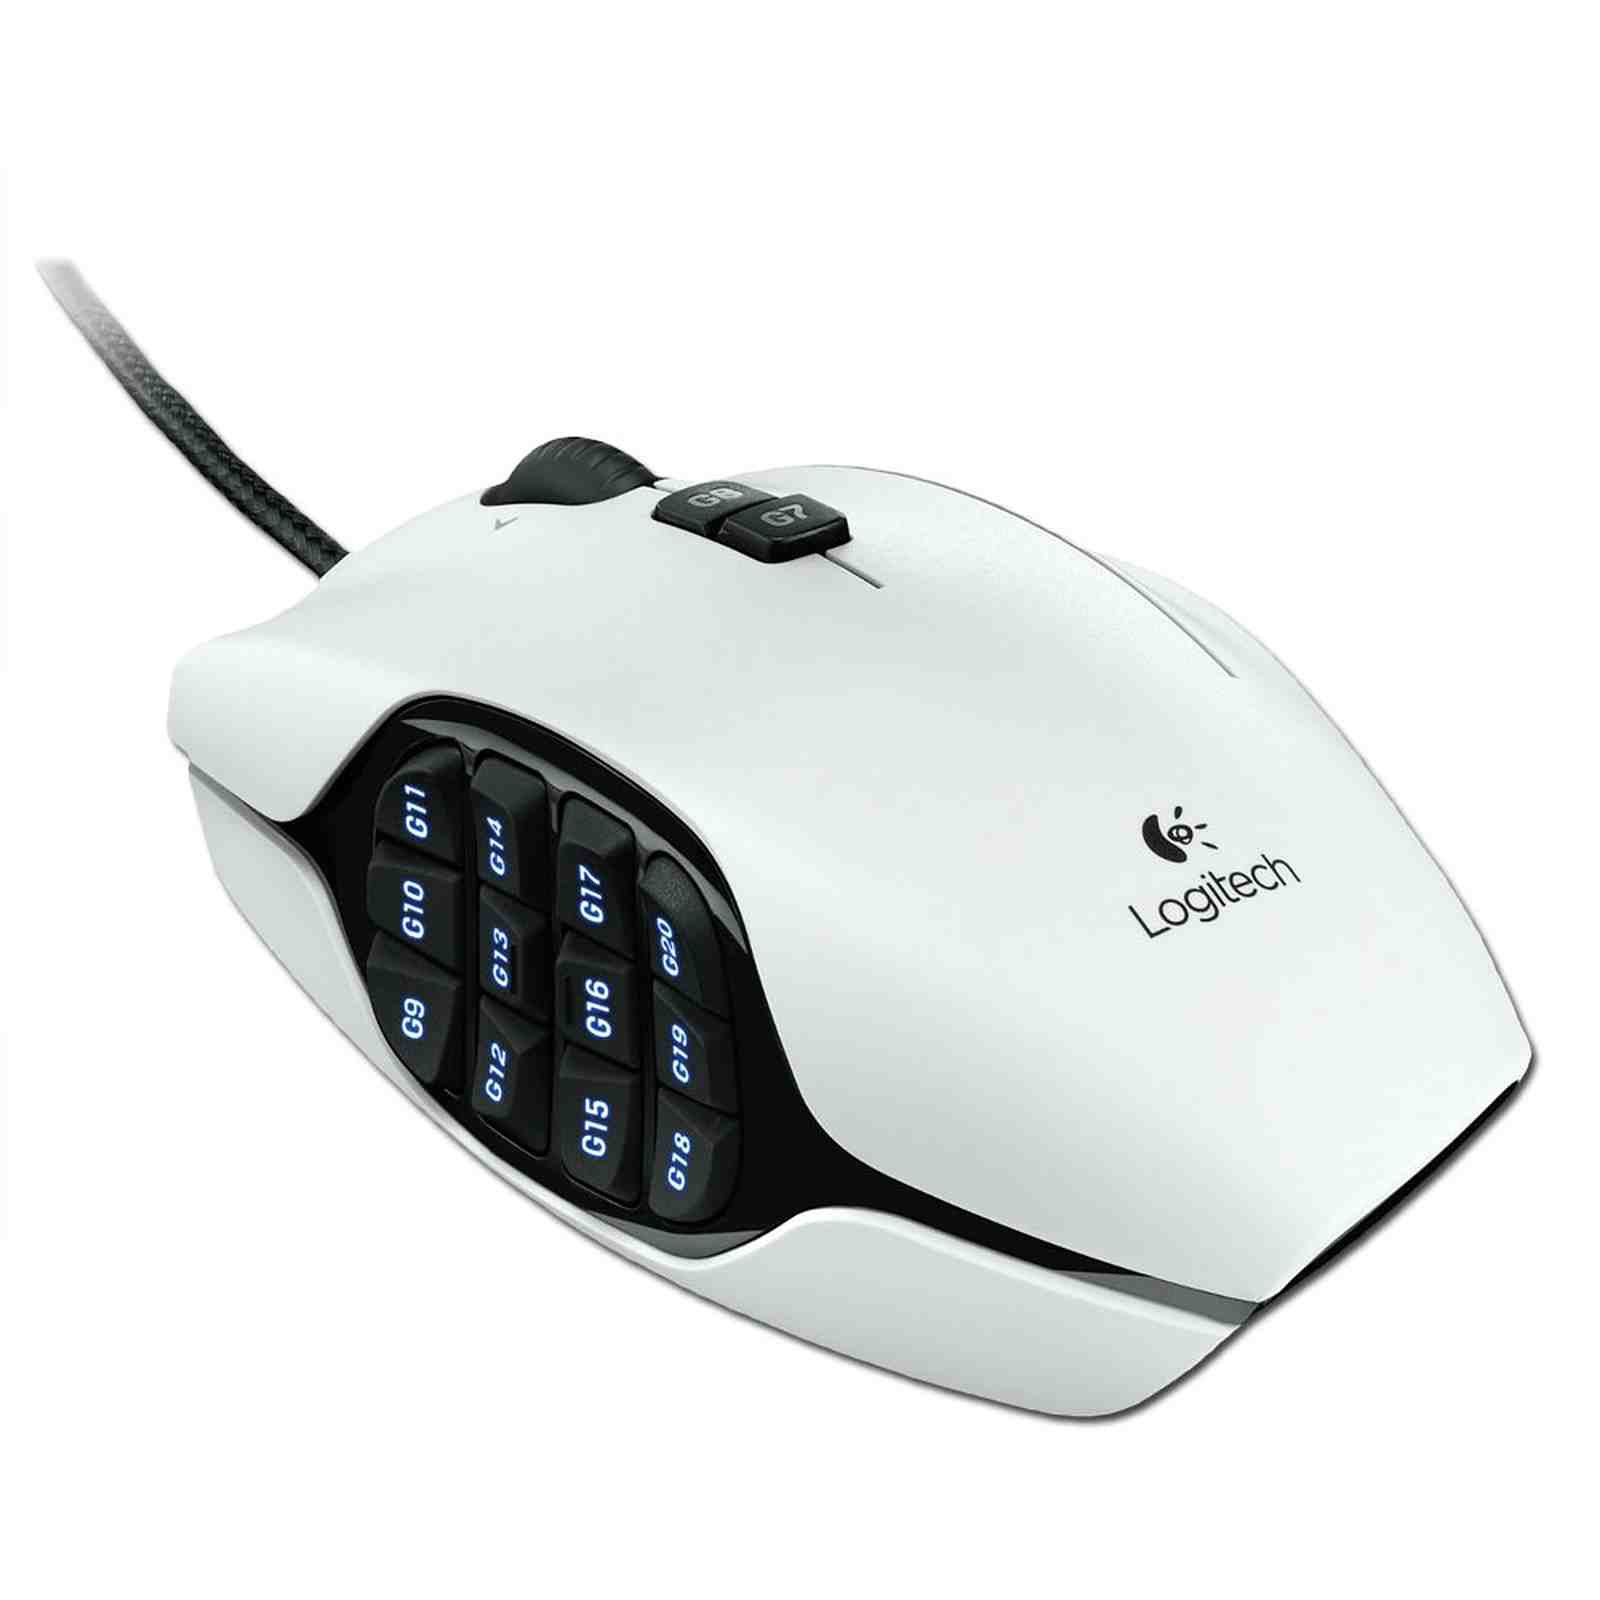
\includegraphics[width=2cm]{Machines/logitech_g600.jpg}
	\caption{\label{fig:logitech_g600}}
	\end{subfigure}
\quad
	\begin{subfigure}[b]{0.2\textwidth}
	\centering
	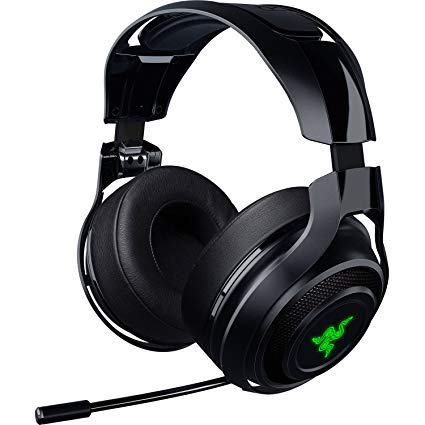
\includegraphics[width=2cm]{Machines/razer_micro_casque.jpg}
	\caption{\label{fig:razer_micro_casque}}
	\end{subfigure}
\quad
	\begin{subfigure}[b]{0.2\textwidth}
	\centering
	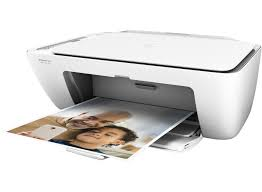
\includegraphics[width=3cm]{Machines/hp_deskjet.jpg}
	\caption{\label{fig:hp_deskjet}}
	\end{subfigure}
\caption{\protect\subref{fig:apple-magic-keyboard-wireless} Clavier, \protect\subref{fig:logitech_g600} souris, \protect\subref{fig:razer_micro_casque} micro-casque, \protect\subref{fig:hp_deskjet} imprimante et scanner.}
\end{figure}
%-------------------------------------------------------------------------------
Concentrons-nous la partie qui reste en général hors de vue, à l'intérieur du boîtier. Les figures~\ref{fig:carte_mere_strix} à~\ref{fig:seasonic_650} montrent des pièces détachées avec lesquelles on va pouvoir assembler un ordinateur.
%-------------------------------------------------------------------------------
\begin{figure}[!htb]
\centering
	\begin{subfigure}[b]{0.22\textwidth}
	\centering
	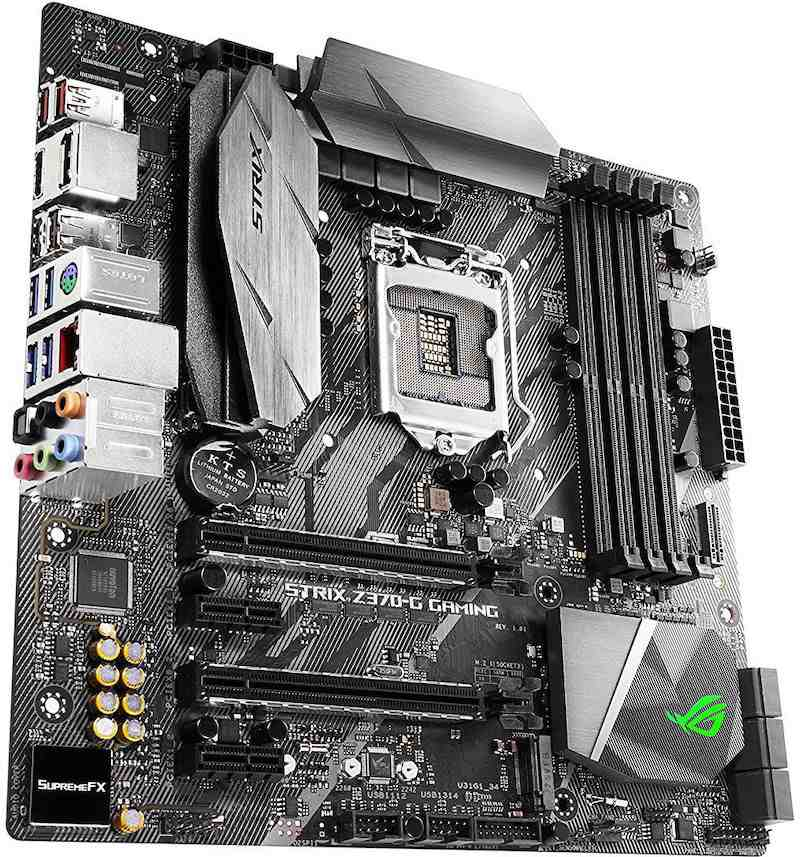
\includegraphics[width=4cm]{Machines/carte_mere_strix.jpg}
	\caption{\label{fig:carte_mere_strix}}
	\end{subfigure}
\quad
	\begin{subfigure}[b]{0.22\textwidth}
	\centering
	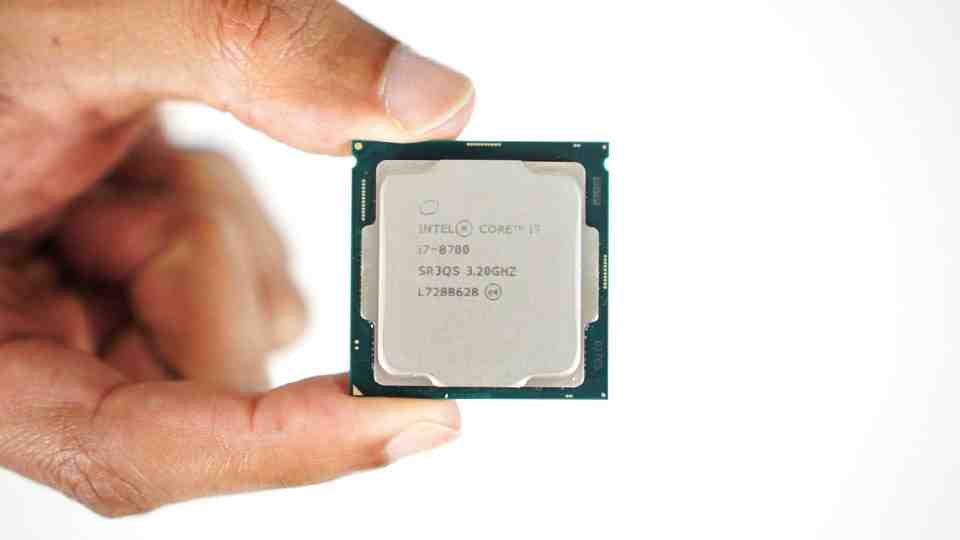
\includegraphics[width=4cm]{Machines/core_i7_8700_hand.jpg}
	\caption{\label{fig:core_i7_8700_hand}}
	\end{subfigure}
\quad
	\begin{subfigure}[b]{0.22\textwidth}
	\centering
	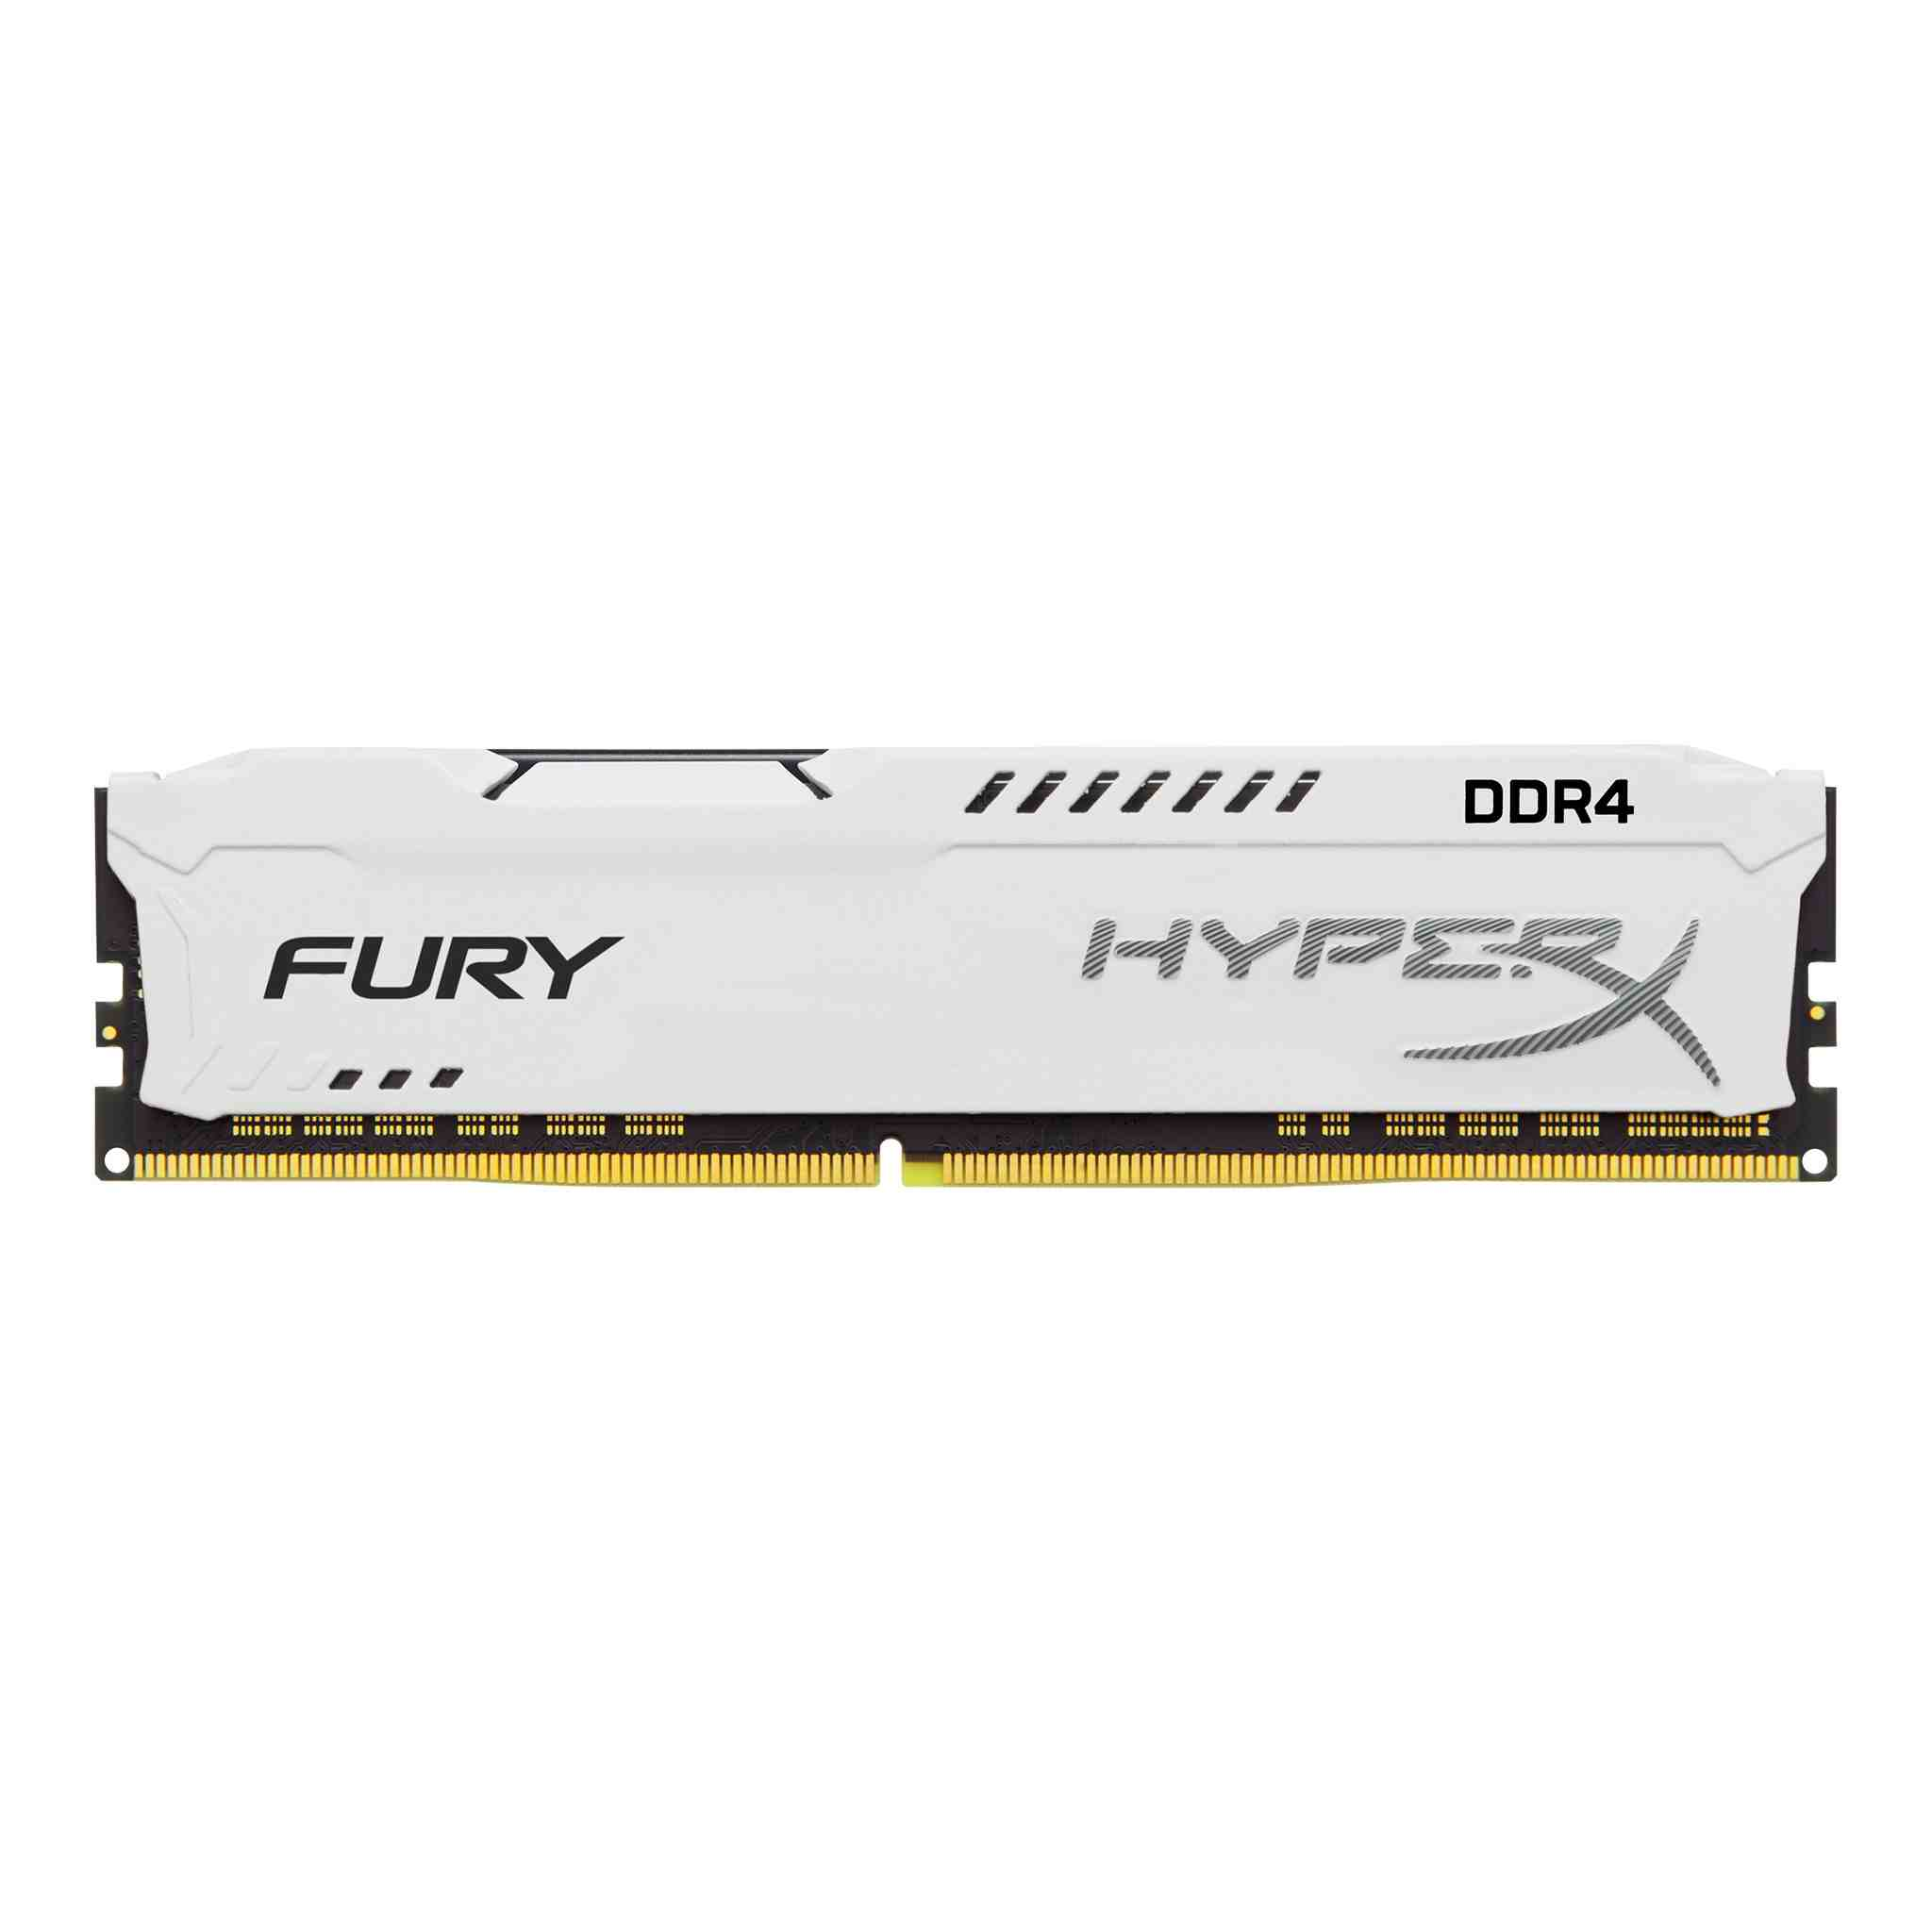
\includegraphics[width=3cm]{Machines/fury_hyperx.jpg}
	\caption{\label{fig:fury_hyperx}}
	\end{subfigure}
\quad
	\begin{subfigure}[b]{0.22\textwidth}
	\centering
	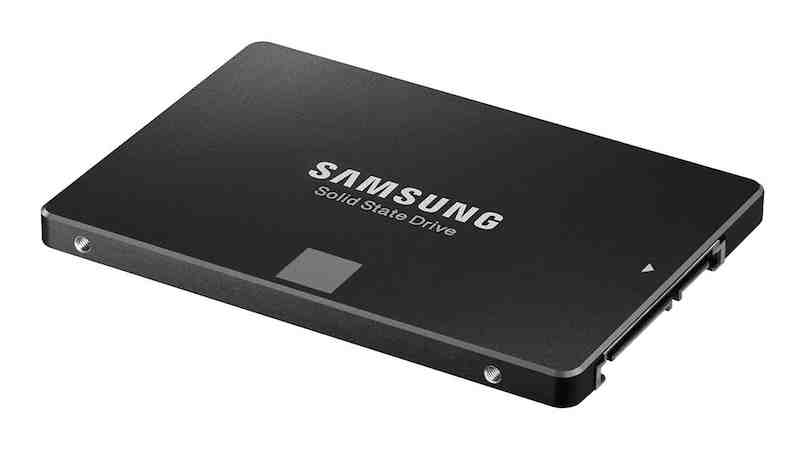
\includegraphics[width=3cm]{Machines/samsung-850-evo.jpeg}
	\caption{\label{fig:samsung-850-evo}}
	\end{subfigure}
\\
	\begin{subfigure}[b]{0.22\textwidth}
	\centering
	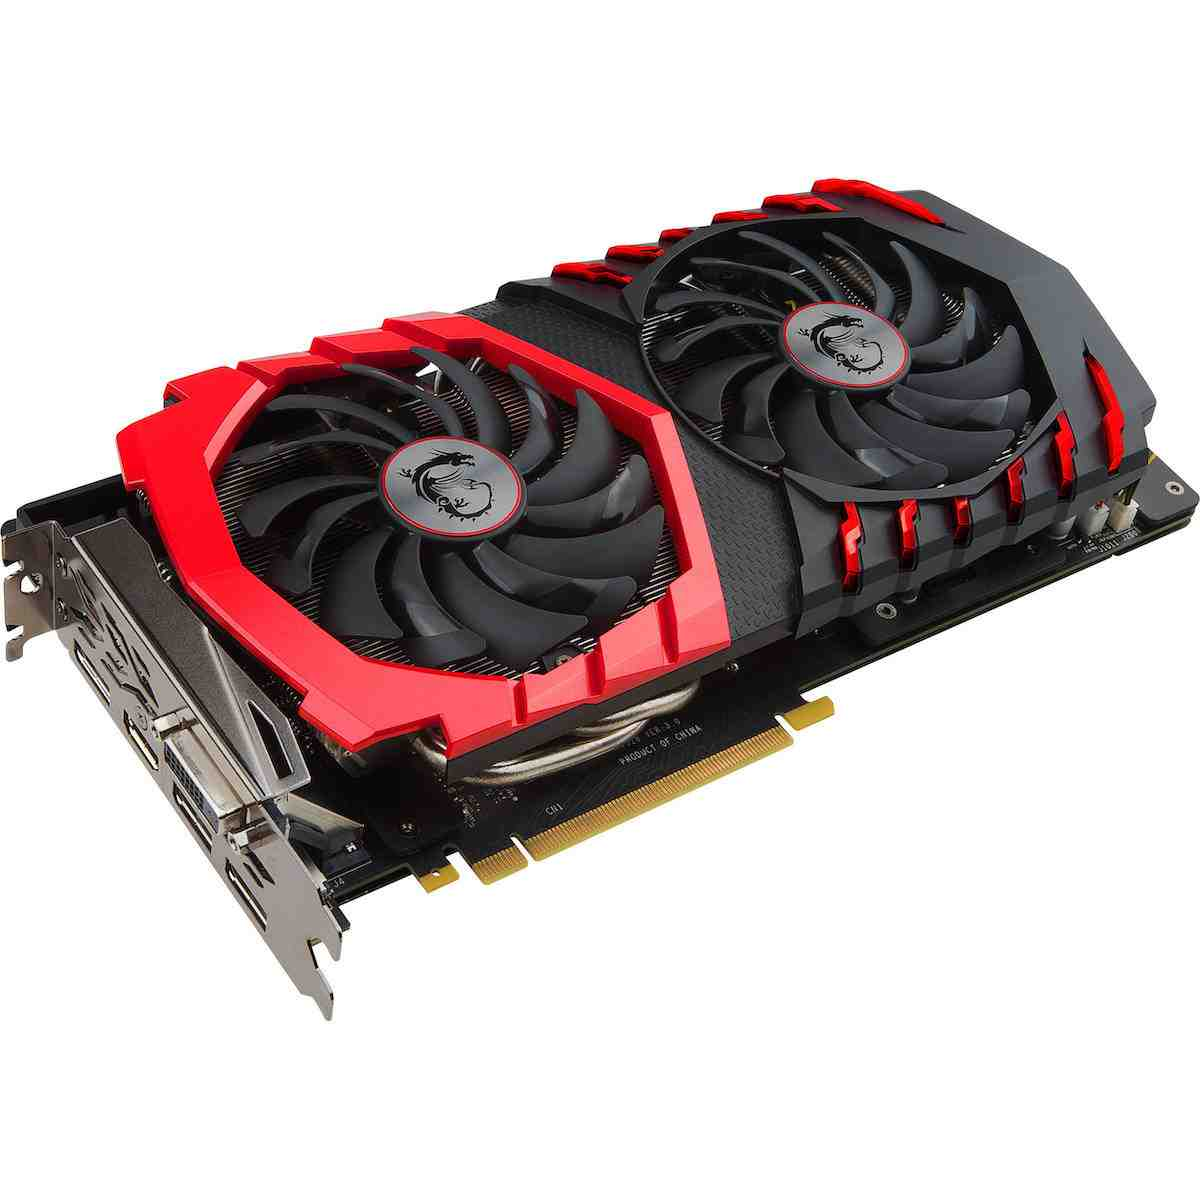
\includegraphics[width=3cm]{Machines/gtx_1060.jpg}
	\caption{\label{fig:gtx_1060}}
	\end{subfigure}
\quad
	\begin{subfigure}[b]{0.22\textwidth}
	\centering
	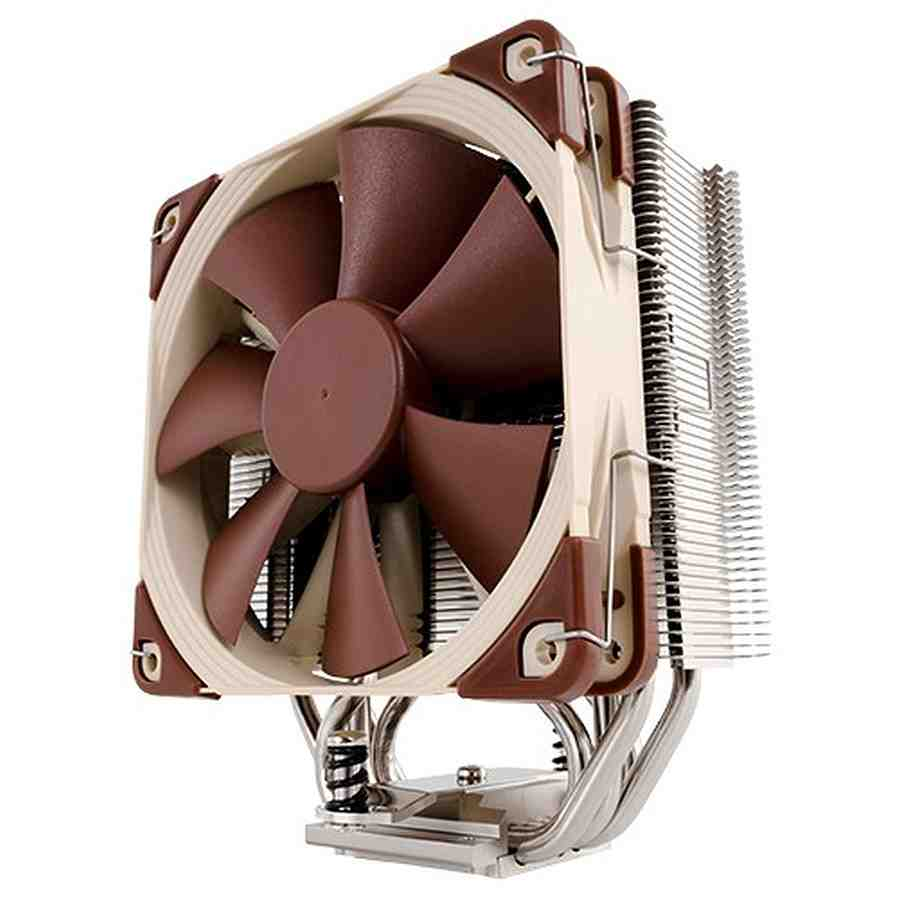
\includegraphics[width=3cm]{Machines/noctua_12s.jpg}
	\caption{\label{fig:noctua_12s}}
	\end{subfigure}
\quad
	\begin{subfigure}[b]{0.22\textwidth}
	\centering
	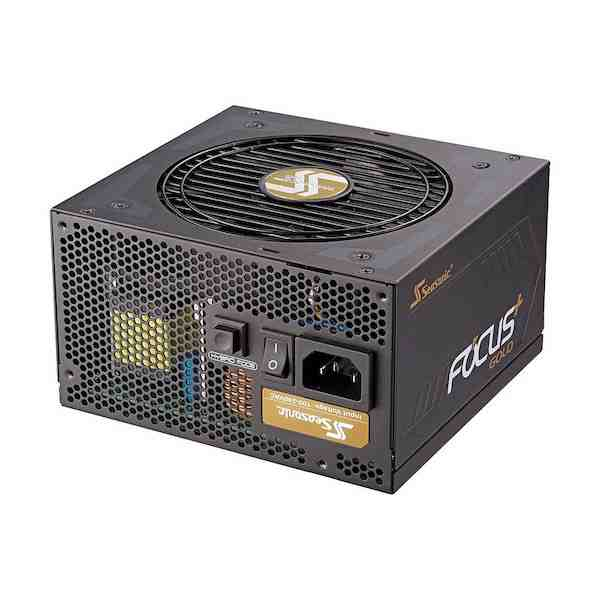
\includegraphics[width=3cm]{Machines/seasonic_650.jpg}
	\caption{\label{fig:seasonic_650}}
	\end{subfigure}
\caption{\protect\subref{fig:carte_mere_strix} Carte-mère, \protect\subref{fig:core_i7_8700_hand} processeur central, \protect\subref{fig:fury_hyperx} barrette de RAM, \protect\subref{fig:samsung-850-evo} disque dur, \protect\subref{fig:gtx_1060} carte graphique, \protect\subref{fig:noctua_12s} dissipateur thermique surmonté d'un ventilateur (\emph{ventirad}), \protect\subref{fig:seasonic_650} alimentation.}
\end{figure}
%-------------------------------------------------------------------------------
Il est intéressant de remarquer que, avec un peu de débrouillardise et de connaissance, il n'est pas difficile de réaliser soi-même l'assemblage d'un ordinateur à partir des ces pièces détachées. Cela ne nécessite en fait pas vraiment de savoir \emph{comment} fonctionne un ordinateur.

Ce fait remarquable résulte de la très grande \emph{normalisation} des ordinateurs : chaque composant réalise des tâches bien déterminées et communique de manière pré-établie, de sorte que l'ordinateur sait précisément quoi lui demander et quoi en attendre, sans que l'utilisateur n'ait à intervenir.
%-------------------------------------------------------------------------------
%-------------------------------------------------------------------------------
\subsection{Et si on les assemble ?}
%-------------------------------------------------------------------------------
%-------------------------------------------------------------------------------
Les pièces ci-dessus, une fois assemblées dans un boîtier adapté, donnent l'ordinateur des figures~\ref{fig:tour1} et~\ref{fig:tour2}. Bien sûr, un tel assemblage n'a rien de compact, et un ordinateur portable ou un téléphone n'est pas fait comme ça. Néanmoins, les éléments constitutifs sont toujours les mêmes. L'exemple traité ici a le mérite de permettre de les observer séparément.
%-------------------------------------------------------------------------------
\begin{figure}[!htb]
\centering
	\begin{subfigure}[b]{0.55\textwidth}
	\centering
	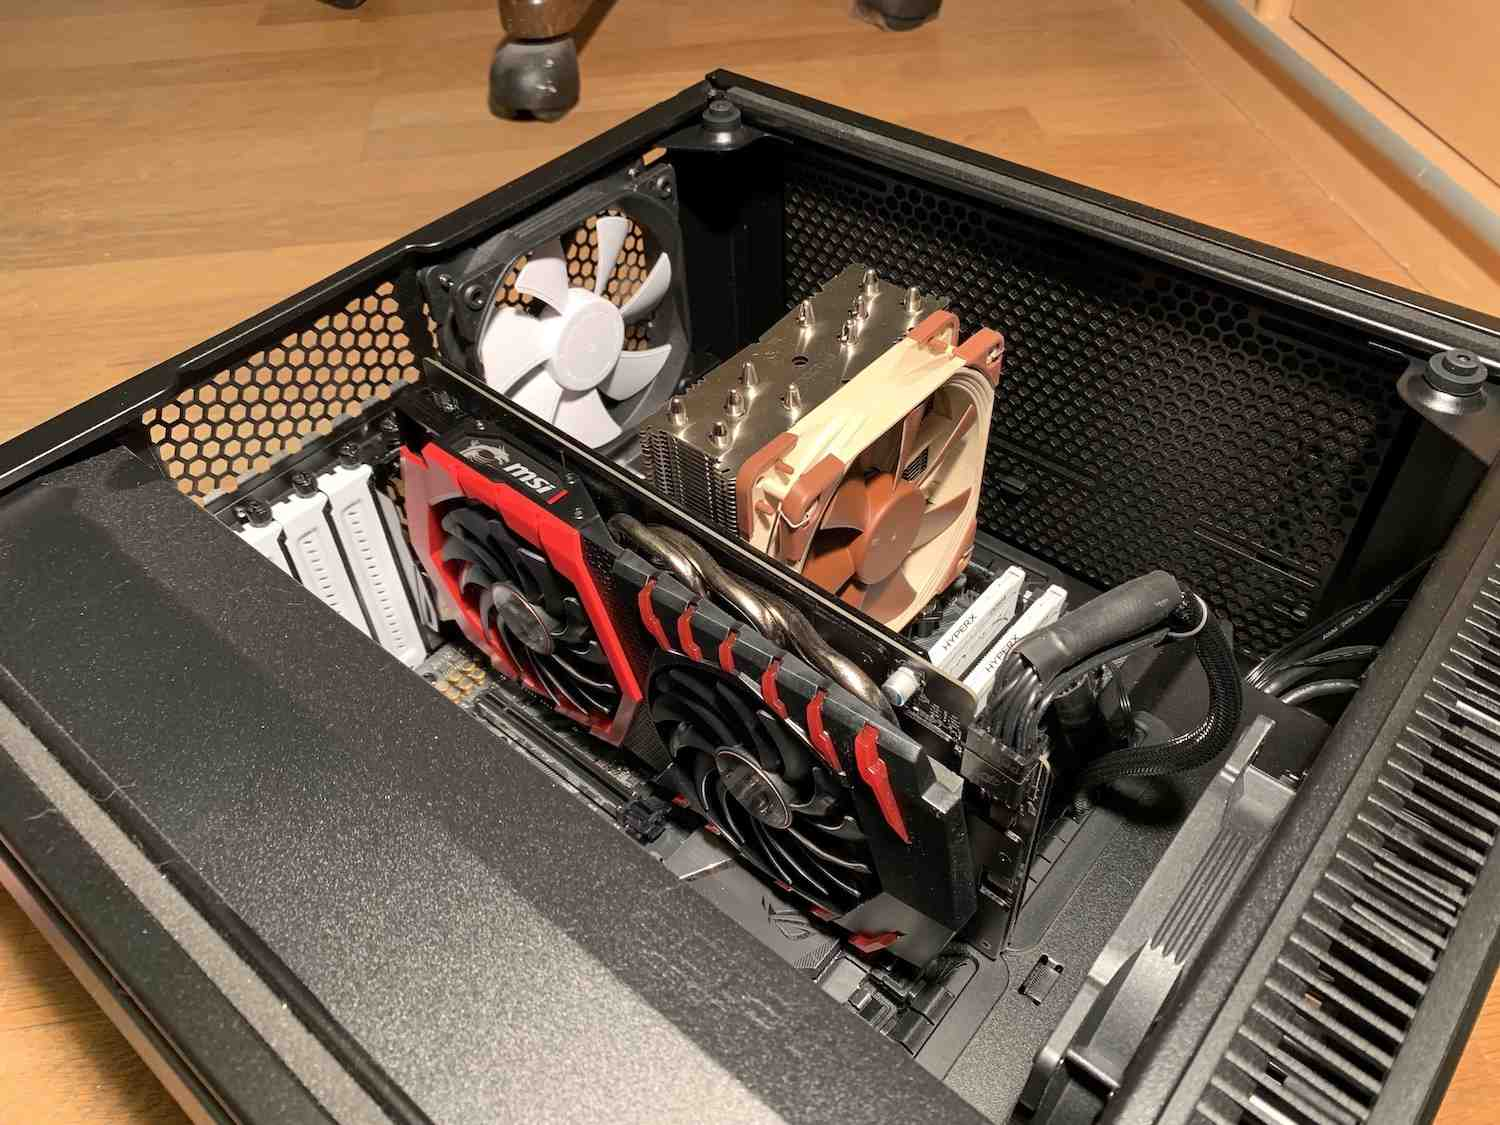
\includegraphics[width=9cm]{Machines/IMG_0328.jpeg}
	\caption{\label{fig:tour1}}
	\end{subfigure}
\quad
	\begin{subfigure}[b]{0.35\textwidth}
	\centering
	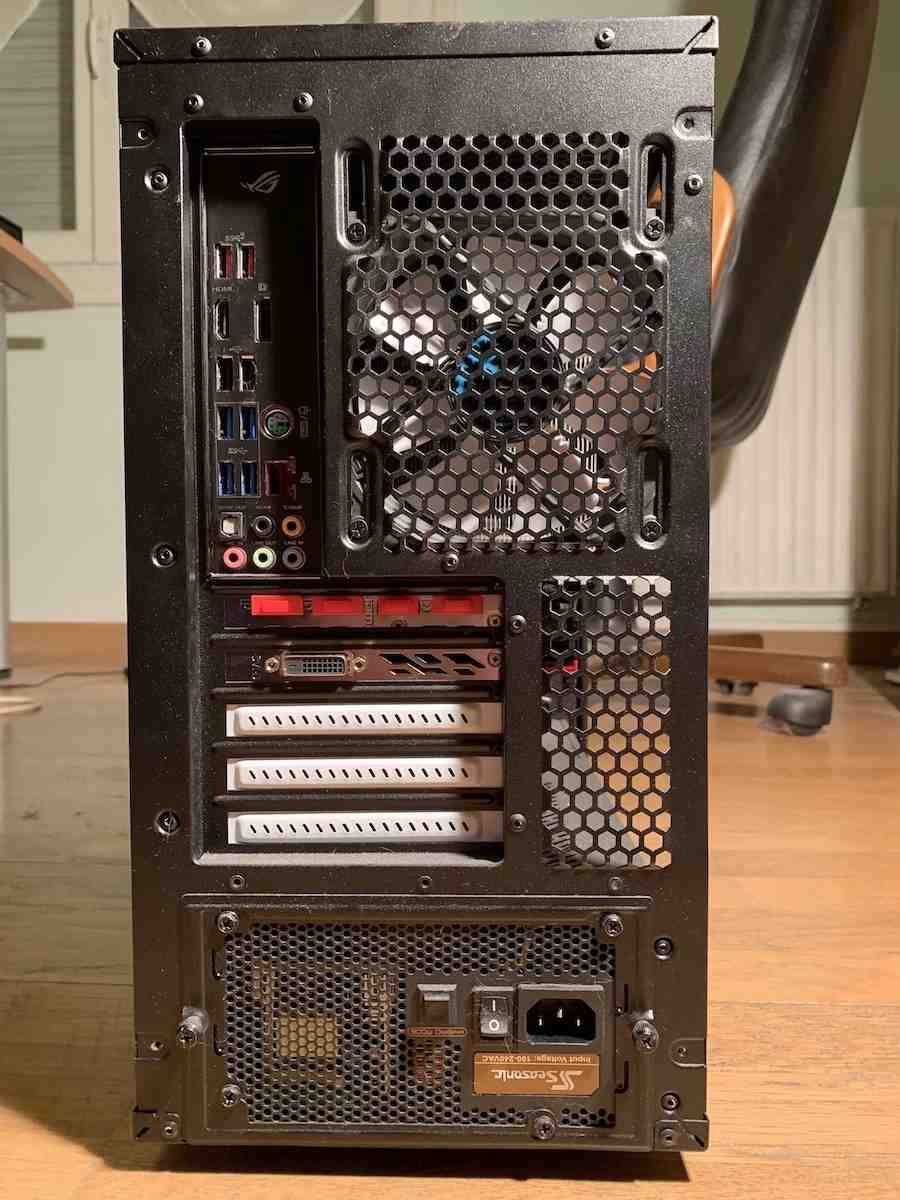
\includegraphics[width=6cm]{Machines/IMG_0324.jpeg}
	\caption{\label{fig:tour2}}
	\end{subfigure}
\caption{Un PC assemblé en tour : \protect\subref{fig:tour1} intérieur, \protect\subref{fig:tour2} arrière.}
\end{figure}
%-------------------------------------------------------------------------------
On remarque que les divers composants sont presque tous connectés à un même élément qui occupe toute la surface d'un flanc de la tour. C'est la \emph{carte-mère} (figure~\ref{fig:carte_mere_strix}), qui joue le rôle de \emph{matrice de communication} : elle comporte de nombreux connecteurs sur lesquels viennent se brancher tous les autres composants et par lesquels ils pourront communiquer entre eux. On y trouve :
	\begin{itemize}
	\item des connecteurs \emph{externes}, en haut à gauche sur la figure~\ref{fig:tour2}, que même les utilisateurs non spécialistes connaissent (USB pour brancher clavier et souris, jack pour brancher des enceintes, etc) ;
	\item des connecteurs \emph{internes}, pour les composants situés à l'intérieur de la tour qui ne sont pas destinés à être branchés et débranchés fréquemment.
	\end{itemize}
Les divers types de connecteurs diffèrent non seulement par leur forme, mais aussi par leurs caractéristiques physiques (électriques, mécaniques ou thermodynamiques). Certains sont optimisés pour laisser passer de gros débits de données, d'autres peuvent transporter des courants électriques intenses pour permettre la recharge d'une batterie, etc.
%-------------------------------------------------------------------------------
%-------------------------------------------------------------------------------
\subsection{Le cheminement des données}
%-------------------------------------------------------------------------------
%-------------------------------------------------------------------------------
Alice\footnote{Dans certains domaines de l'informatique, on a estimé peu conviviales les appellations «utilisateur A» et «utilisateur B» dans les exemples, et de là est née la tradition de les appeler Alice et Bob.} vient de saisir un texte et elle tape le raccourci clavier déclenchant sa sauvegarde sur le disque dur de l'ordinateur. Elle s'attend donc à deux choses : d'abord que son document soit enregistré, ensuite qu'il y en ait une confirmation visuelle à l'écran. Quel est le chemin pris par les données au cours de cette opération ?
%-------------------------------------------------------------------------------
\subsubsection{Un peu de vocabulaire}
%-------------------------------------------------------------------------------
Quand un composant peut communiquer avec d'autres, il dispose d'un \emph{contrôleur}. C'est un élément électronique qui sert d'interface avec l'extérieur et orchestre les communications.

Comme les flux de données allant d'un composant à l'autre peuvent entrer ou sortir des composants, on parle de flux d'\emph{entrée/sortie} ou I/O (pour Input/Output).

Bien que ce ne soit pas une règle absolue, on classe en général les I/O en deux catégories, les «lents» et les «rapides», qui ne sont pas gérées par les mêmes contrôleurs.

Le canal de communication entre deux composants s'appelle un \emph{bus}.
%-------------------------------------------------------------------------------
\subsubsection{Exemple}
%-------------------------------------------------------------------------------
\begin{figure}[!htb]
\centering
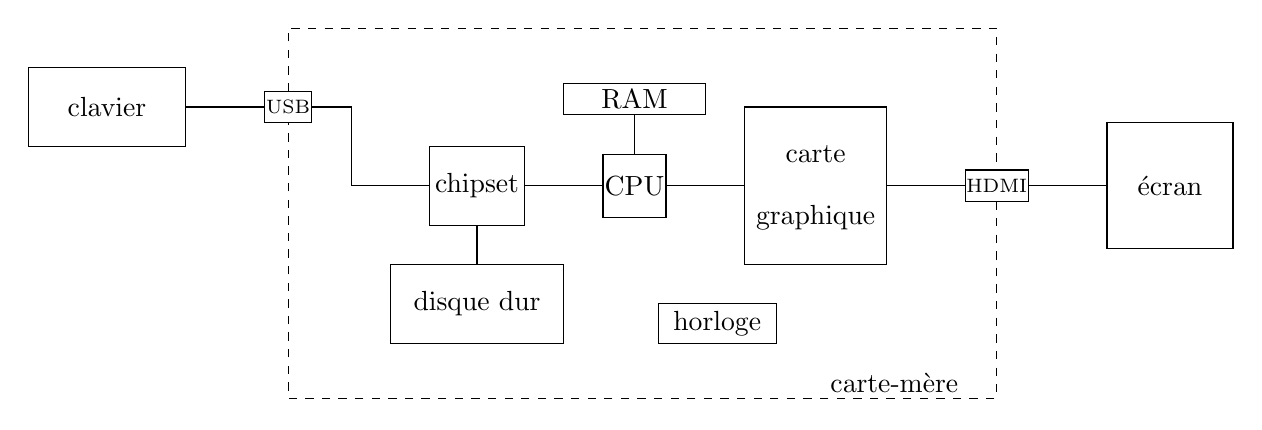
\begin{tikzpicture}
% Clavier
\draw (0,0) rectangle (2,1);
\node at (1,0.5){clavier};
\draw (2,0.5)--++(1,0);
% USB
\draw (3,0.3) rectangle (3.6,0.7);
\node at (3.3,0.5){\scriptsize USB};
\draw (3.6,0.5)--++(0.5,0)--++(0,-1)--++(1,0);
% Chipset
\draw (5.1,-1) rectangle (6.3,0);
\node at (5.7,-0.5){chipset};
% SATA
\draw (5.7,-1)--++(0,-0.5);
\draw (4.6,-1.5) rectangle (6.8,-2.5);
\node at (5.7,-2){disque dur};
% CPU
\draw (6.3,-0.5)--++(1,0);
\draw (7.3,-0.9) rectangle (8.1,-0.1);
\node at (7.7,-0.5){CPU};
% RAM
\draw (7.7,-0.1)--++(0,0.5);
\draw (6.8,0.4) rectangle (8.6,0.8);
\node at (7.7,0.6){RAM};
% Carte graphique
\draw (8.1,-0.5)--++(1,0);
\draw (9.1,-1.5) rectangle (10.9,0.5);
\node at (10,-0.1){carte};
\node at (10,-0.9){graphique};
% HDMI
\draw (10.9,-0.5)--++(1,0);
\draw (11.9,-0.7) rectangle (12.7,-0.3);
\node at (12.3,-0.5){\scriptsize HDMI};
% Écran
\draw (12.7,-0.5)--++(1,0);
\draw (13.7,-1.3) rectangle (15.3,0.3);
\node at (14.5,-0.5){écran};
% Carte-mère
\draw[dashed] (3.3,0.7)--(3.3,1.5)--(12.3,1.5)--(12.3,-0.3);
\draw[dashed] (12.3,-0.7)--(12.3,-3.2)--(3.3,-3.2)--(3.3,0.3);
\node at (11,-3){carte-mère};
% Horloge
\draw (8,-2.5) rectangle (9.5,-2);
\node at (8.75,-2.25){horloge};
\end{tikzpicture}
\caption{\label{fig:chemin_données}Architecture typique d'un ordinateur personnel (bien sûr, il existe des variantes).}
\end{figure}
%-------------------------------------------------------------------------------
Suivons les flux de données sur le schéma de la figure~\ref{fig:chemin_données}. 

Sur la carte-mère, les contrôleurs I/O «lents» sont regroupés dans le chipset,\footnote{Le contrôleur lui-même s'appelle le \emph{southbridge}.} tandis que les contrôleurs I/O «rapides» sont dans le CPU.\footnote{Collectivement appelées \emph{northbridge}.}

Gardez en tête que les diverses étapes ci-dessous ne se font pas toutes seules. Le système d'exploitation intervient fortement pour traiter les données et coordonner leurs échanges. 
%-------------------------------------------------------------------------------
\begin{enumerate}
	\item L'information «une touche du clavier a été pressée» arrive donc par le connecteur (typiquement USB) sur lequel le clavier est branché. 
	
	 Ce flux est donc reçu par le contrôleur situé dans le chipset.
	
	Mais l'histoire ne s'arrête pas là : l'écran n'est pas relié au chipset, l'endroit où est mémorisé le document d'Alice non plus, et l'ordinateur ne comprend pas «automatiquement» ce que veulent dire les touches enfoncées par Alice\dots
	\item L'information est envoyée vers le contrôleur du \emph{processeur central} (CPU, représenté seul figure~\ref{fig:core_i7_8700_hand} et caché sous le ventilateur central sur la figure~\ref{fig:tour1}). 
	
	Une fois qu'il a reçu notre flux de données, le processeur va devoir faire des calculs pour les traiter, afin de comprendre et d'accomplir sa tâche. Mais pour cela, dans quelle partie de l'ordinateur se trouve le document tant qu'il n'a pas été enregistré ?
	\item La réponse est, dans la \emph{mémoire vive} (RAM : Random Access Memory). Composant rapide relié au processeur, cet espace de stockage est caractérisé par sa volatilité.\footnote{Les données n'y sont pas stockées durablement. Une coupure de courant même très brève suffit à perdre tout son contenu, comme beaucoup de gens en ont déjà fait l'amère expérience !} La RAM se présente physiquement sous la forme de barrettes, comme représenté figure~\ref{fig:fury_hyperx} et que l'on voit à droite du processeur sur la figure~\ref{fig:tour1}.
	\item Le CPU doit maintenant orchestrer le transfert des données depuis la RAM vers le disque dur\footnote{En toute rigueur, l'appellation de «disque» n'est plus vraiment appropriée, les nouveaux modèles ne comportant plus de plateau tournant, ni même la moindre pièce mobile. Il vaut mieux parler de lecteur (\emph{drive} en Anglais).} (figure~\ref{fig:samsung-850-evo}). Ce dernier est bien sûr un dispositif de stockage ; comparé à la RAM, il est notablement plus lent mais les données y sont \emph{persistantes} (elles survivent à une coupure de courant). S'il est d'un modèle courant, le disque dur est connecté au contrôleur du chipset. Le document d'Alice est enfin enregistré !
	\item Reste à mettre à jour l'affichage pour informer Alice que l'enregistrement a été effectué. Le CPU possède aussi un contrôleur relié à la \emph{carte graphique}, représentée figure~\ref{fig:gtx_1060}. Composant très complexe capable de mener ses propres calculs, c'est sur elle que l'écran est branché : elle s'occupe donc du traitement et de la mise en forme des données vidéo.\footnote{Par le passé, le CPU s'en occupait directement, mais c'est une tâche intensive faisant appel à des méthodes de calcul très spécifiques, de sorte qu'on préfère en général la déporter vers une unité de calcul dédiée, la \emph{carte graphique}.}
\end{enumerate}
%-------------------------------------------------------------------------------
Notons que la plupart de ces opérations sont menées en suivant un rythme précis fourni par un composant de la carte-mère appelé \emph{horloge}.
%-------------------------------------------------------------------------------
%-------------------------------------------------------------------------------
\subsection{L'horloge}
%-------------------------------------------------------------------------------
%-------------------------------------------------------------------------------
\begin{wrapfigure}{r}{4.5cm}
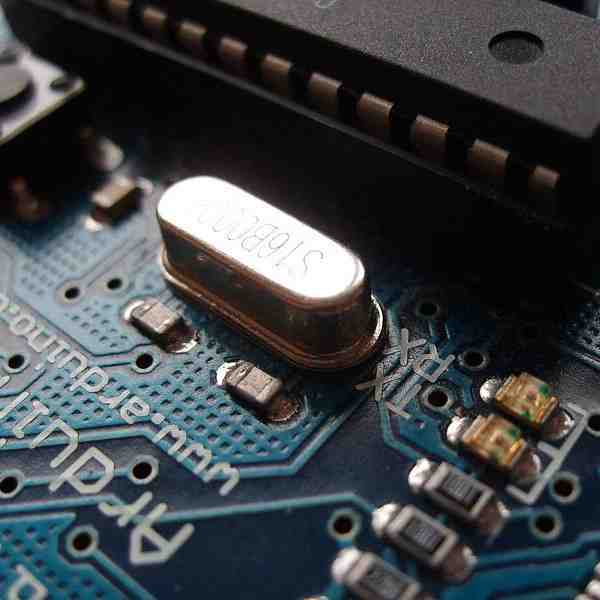
\includegraphics[width=3.5cm]{Machines/quartz-crystal.jpg}
\caption{\label{fig:quartz-crystal}Horloge dans la carte-mère.}
\end{wrapfigure}
Ce composant situé sur la carte-mère (figure~\ref{fig:quartz-crystal}) contient un cristal piézoélectrique. Ce matériau possède deux caractéristiques spécifiques :
	\begin{itemize}
	\item C'est un oscillateur mécanique, capable de se contracter et de se dilater à une fréquence qui lui est propre (sa \emph{fréquence de résonance}, déterminée par sa fabrication).
	\item Quand il est soumis à une tension électrique, il réagit en se mettant à osciller mécaniquement. Réciproquement, quand il oscille mécaniquement, il produit une tension oscillante à ses bornes.
	\end{itemize}
L'astuce est de prélever la tension qu'il produit par ses oscillations mécaniques naturelles, de l'amplifier et de la réappliquer à ses bornes, ce qui «régénère» les oscillations mécaniques. Si l'amplification est suffisante pour compenser les pertes énergétiques, les oscillations deviennent \emph{entretenues} et le cristal devient la source d'un signal parfaitement périodique sur lequel beaucoup d'opérations se calent.
%-------------------------------------------------------------------------------
%-------------------------------------------------------------------------------
\subsection{Considérations thermiques}
%-------------------------------------------------------------------------------
%-------------------------------------------------------------------------------
Il est bien connu qu'un composant électronique a tendance à chauffer. Plus il est sollicité, plus il est amené à travailler vite, et les courants électriques circulant dedans produisent de la chaleur par effet Joule. Une température excessive peut perturber les calculs et, dans des cas extrêmes, endommager le composant.\footnote{Heureusement, beaucoup de composants sont munis de sondes thermiques pour se désactiver automatiquement en cas de surchauffe.}

À titre d'exemple, le dégagement de chaleur d'un processeur de moyenne gamme en pleine charge peut approcher 100 W, avec une température atteignant les 80\degre\footnote{Les processeurs destinés à des machines intégrées, comme des ordinateurs portables ou des smartphones, sont conçus pour dégager beaucoup moins, au prix souvent de performances réduites.}. On comprend que, dans les entreprises, les salles informatiques soient thermo-régulées !\footnote{Et si l'ordinateur est en plus muni d'une carte graphique puissante, le dégagement thermique peut être doublé, voire triplé.}

Les figures~\ref{fig:tour1} et~\ref{fig:tour2} montrent les points clefs de la stratégie de gestion des flux thermiques :
%-------------------------------------------------------------------------------
\begin{itemize}
	\item Tous les composants dégageant de la chaleur (carte graphique, processeur central, chipset) sont coiffés d'une pièce métallique appelée \emph{dissipateur thermique} (figure~\ref{fig:noctua_12s}). Très bon conducteur thermique et taillé en multiples ailettes pour maximiser sa surface de contact avec l'air ambiant, il conduit la chaleur vers un ventilateur qui l'évacue vers l'intérieur de l'ordinateur.
	\item La tour elle-même est munie d'un ou plusieurs ventilateurs qui pompent la chaleur dégagée par les ventilateurs précédents et l'éjectent à l'extérieur du boîtier.	\item L'ordinateur est branché sur le secteur et reçoit donc du 220 V alternatif, alors que les composants nécessitent une tension bien plus faible et continue. Il faut donc une \emph{alimentation} (figure~\ref{fig:seasonic_650}) qui va s'occuper de la conversion. Cela génère de la chaleur, ainsi qu'un rayonnement électromagnétique capable de perturber son environnement dans un rayon de quelques centimètres. L'alimentation est donc en général éloignée du reste de l'ordinateur (on la voit tout en bas de la figure~\ref{fig:tour2}).
\end{itemize}
%-------------------------------------------------------------------------------
%-------------------------------------------------------------------------------
\section{Coder l'information}
%-------------------------------------------------------------------------------
%-------------------------------------------------------------------------------
\subsection{Exprimer une quantité d'information}
%-------------------------------------------------------------------------------
%-------------------------------------------------------------------------------
L'unité élémentaire d'information est le bit (binary digit, chiffre binaire). Il n'a donc que deux valeurs possibles, 0 ou 1. 

Un groupement de $8=2^3$~bits s'appelle un \emph{octet} (\emph{byte} en Anglais), de symbole B.\footnote{En France, on trouve souvent la notation o à la place de B, mais elle n'est pas reconnue internationalement.}

On peut définir des multiples de l'octets comme pour n'importe quelle unité (par des puissances de 10), mais comme en informatique on travaille toujours en base 2, on peut aussi les définir par des puissances de 2. Remarquant que $2^{10}= 1024$ :
%-------------------------------------------------------------------------------
\begin{center}
\begin{tabular}{lc|lc}
Unité (base 2) & Valeur & Unité (base 10) & Valeur\\
\hline
kibi-octet (kiB) & 1024 B & kilo-octet (kB) & 1000 B\\
mébi-octet (MiB) & 1024 kiB & méga-octet (MB) & 1000 kB\\
gibi-octet (GiB) & 1024 MiB & giga-octet (GB) & 1000 MB\\
tébi-octet (TiB) & 1024 GiB & téra-octet (TB) & 1000 GB
\end{tabular}
\end{center}
%-------------------------------------------------------------------------------
Enfin, attention aux confusions de la langue courante. Par écrit les deux systèmes de notation sont globalement respectés (en tout cas dans le monde professionnel), à l'oral on a tendance à utiliser les appellations de la base 10 même quand on parle de la base 2. Donc prêtez attention au contexte !
%-------------------------------------------------------------------------------
%-------------------------------------------------------------------------------
\subsection{Codage des valeurs}
%-------------------------------------------------------------------------------
%-------------------------------------------------------------------------------
La manière dont est traduite une valeur en bits dépend de la nature de la variable, son {\bf type}. 

Le nombre de bits alloués  gouverne le nombre maximal de valeurs différentes qui peuvent être utilisées. Les valeurs les plus courantes sont
	\begin{center}
	\begin{tabular}{cl}
	Espace alloué & Nombre de valeurs différentes\\
	\hline
	8  bits & $2^8=256$\\
	10  bits & $2^{10}=10\,24$\\
	12  bits & $2^{12}=40\,96$\\
	16  bits & $2^{16}=65\,536$\\
	24  bits & $2^{24}=16\,777\,216$\\
	32  bits & $2^{32}=4\,294\,967\,296$\\
	64  bits & $2^{64}=18\,446\,744\,073\,709\,551\,616$
	\end{tabular}
	\end{center}
Voici quelques utilisations typiques :
	\begin{itemize}
	\item 8  bits : codage d'une couleur dans les formats d'images et de vidéos (JPEG, Blu-ray \dots)
	\item 10  bits : code d'une couleur dans certains formats d'images professionnels.
	\item 16  bits : codage des sons dans les formats audio grand public (CD, MP3 \dots)
	\item 24  bits : codage des sons dans les formats audio professionnels (mastering).
	\item 32  bits : codage des entiers dans la plupart des langages de programmation.
	\item 64  bits : codage des flottants dans la plupart des langages de programmation.
	\end{itemize}
	

Les types simples les plus utilisés sont les entiers, les flottants et les caractères.
%-------------------------------------------------------------------------------
\subsubsection{Entiers}
%-------------------------------------------------------------------------------
%-------------------------------------------------------------------------------
En première approche, on peut dire que les entiers sont stockés sous forme binaire dans l'espace mémoire alloué : l'entier $n$ est représenté sur $p$ bits par la suite $(a_{p-1},a_{p-2},\ldots,a_1,a_0)$ de valeurs 0 ou 1 telle que $\displaystyle n = \sum_{k=0}^{p-1}a_k 2^k$\footnote{C'est la représentation {\bf big endian} ou {\bf petitboutienne}, d'autres ordres des indices existent.}.

Il reste le problème de la représentation des entiers négatifs, nous y reviendront dans un chapitre ultérieur.

Cela limite les entiers à un intervalle de taille $2^p$. Cependant, en théorie, Python est capable d'utiliser les entiers sans limite de valeur.
%-------------------------------------------------------------------------------
\subsubsection{Flottants}
%-------------------------------------------------------------------------------
La notion mathématique de réel n'a pas d'équivalent  en informatique. En effet un nombre réel nécessite souvent un  processus infini pour être défini (suite de ses décimales, suite qui tend vers le réel, etc) qu'on ne peut pas contenir dans une mémoire finie. On devra se contenter d'approximations. 

Les valeurs approchant les nombres réels sont appelés {\it nombres flottants} pour rappeler que leur virgule «flotte», leur forme est semblable à la notation scientifique utilisée dans les sciences, par exemple $6,02 10^23$. 
Si on suppose que l'on dispose de 8 chiffres significatifs le nombre précédent s'écrit $\displaystyle  \frac{60200000}{10^7}10^{30}$, il peut être représenté par les entiers 60200000 et 30.

En Python, ces valeurs ont le type \type{float}. On les écrit avec un point à la place de notre virgule ; on peut aussi utiliser un exposant \type{e} qui signifie puissance 10 ; 
\type{898547e-5} signifie \type{8.98547}

Leur codage en mémoire utilise deux entiers, comme l'exemple ci-dessus que nous étudierons dans un chapitre ultérieur.
%-------------------------------------------------------------------------------
\subsubsection{Caractères}
%-------------------------------------------------------------------------------
De même chaque caractère est associé à un nombre entier que l'on peut coder dans la mémoire.

Il faut donc une table de correspondance entre les caractères et leurs représentations entières. Cela s'appelle un \emph{encodage}.


{\bf L'encodage ASCII}
Le plus ancien encodage encore utilisé, l'ASCII 7  bits, ne contient que les caractères utilisés en Anglais. ASCII veut dire American Standard Code for Information Interchange : Code américain normalisé pour l'échange d'information.

Il contient $128=2^7$ caractères, donc chaque caractère peut être représenté par un entier sur 7  bits. En pratique, l'unité élémentaire d'information en mémoire étant l'octet, un caractère se voit donc plutôt allouer 8  bits, le 8\ieme{} bit étant alors laissé à 0.

On y trouve les 26 lettres de l'alphabet latin en majuscules et minuscules, les principaux symboles de ponctuation et les chiffres arabes. Quelques exemples :
	\begin{center}
	\begin{tabular}{cc|cc}
	Caractère & Code & Caractère & Code\\
	\hline
	A & 65 & 0 & 48\\
	B & 66 & 1 & 49\\
	a & 97 & ( & 40
	\end{tabular}
	\end{center}
Il y a aussi des «caractères spéciaux» qui n'ont pas d'apparence mais sont utiles par exemple pour structurer une chaîne de caractères :
	\begin{center}
	\begin{tabular}{lcc}
	Caractère & Code & Représentation en Python\\
	\hline
	Nouvelle ligne & 10 & \verb|\n|\\
	Tabulation & 9 & \verb|\t|
	\end{tabular}
	\end{center}

Par contre, l'ASCII 7  bits ne contient pas de caractères accentués, de lettres grecques, etc.\footnote{Ces limitations se retrouvent encore aujourd'hui, par exemple, dans certains communications par internet : il est bien connu qu'utiliser des lettres accentuées dans des mails ou des noms de fichier quand on communique avec des gens d'autres pays peut parfois créer des problèmes.} Du coup, dans la deuxième moitié du 20\ieme{} siècle, chaque pays a utilisé le 8\ieme{} bit pour étendre l'ASCII et y ajouter les caractères nécessaires pour sa ou ses langues.

Mais ces efforts n'ont pas été normalisés, conduisant à de multiples encodages variant selon les pays et les types d'ordinateurs, générant un casse-tête d'interopérabilité.


{\bf L'Unicode}
Il a fallu attendre les années 2000 pour voir se concrétiser un standard international recouvrant la grande majorité des besoins de toutes les langues : l'Unicode. De nos jours, l'Unicode est l'encodage par défaut de la majorité des ordinateurs usuels.

Tous les langages de programmation modernes savent manipuler des caractères en Unicode.\footnote{Python, depuis sa version 3, travaille nativement en Unicode.} Dans la variante UTF-8 de l'Unicode (la plus répandue), l'espace mémoire alloué à un caractère est variable, allant de 1 à 4 octets.

La distinction se fait sur les premiers bits :
	\begin{itemize}
	\item Si le premier bit est 0, alors le caractère occupe un octet. Il reste 7 bits pour le caractère lui-même, qui est alors encodé suivant la table ASCII 7  bits.
	\item Si les trois premiers bits sont 110, alors il occupe 2 octets. L'octet suivant doit alors commencer par 10 (bits de continuité), ce qui laisse un total de 11 bits pour le caractère. Cette plage contient les caractères latins absents de l'Anglais, mais aussi d'autres alphabets (grec, hébreu, cyrillique, arabe\dots) Exemples :
		\begin{center}
		\begin{tabular}{cc}
		Caractère & Code\\
		\hline
		¿ & \underline{110}00010~\underline{10}111111\\
		É & \underline{110}00011~\underline{10}001001\\
		$\mathrm{\psi}$ & \underline{110}01111~\underline{10}001000
		\end{tabular}
		\end{center}
	\item Si les quatre premiers bits sont 1110, alors il occupe 3 octets. Retirant les bits de continuité, cela laisse 16 bits pour le caractère. On y trouve encore d'autres alphabets, le Braille, des écritures idéographiques comme le Chinois ou le Japonais, mais aussi les célèbres caractères Dingbats, des symboles de ponctuation et des symboles mathématiques. Exemples :
		\begin{center}
		\begin{tabular}{cc}
		Caractère & Code\\
		\hline
%		月 & \underline{1110}0010~\underline{10}111101~\underline{10}001001\\
		$\oint$ & \underline{1110}0010~\underline{10}001000~\underline{10}101110
		\end{tabular}
		\end{center}
	\item Si les cinq premiers bits sont 11110, alors il occupe 4 octets, ce qui laisse 21 bits pour le caractère. On y trouve des langues anciennes, les notations musicales, et encore plus de symboles, en particulier les célèbres emoji.\footnote{On passe ici sous silence le mécanisme de \emph{combinaison} de caractères en Unicode, nécessaire pour les emoji.}
	\end{itemize}

En fin de compte, la représentation Unicode permet d'inclure des \emph{millions} de caractères différents. La majorité des valeurs binaires correspondantes ne sont d'ailleurs pas encore utilisées à ce jour.

Cette variabilité de l'espace mémoire alloué peut compliquer les traitements informatiques, mais elle permet de garder la compatibilité avec l'ASCII tout en optimisant l'espace mémoire occupé par une chaîne de caractères (inutile de prendre 4 octets par caractère si on n'écrit qu'en Français !)
%-------------------------------------------------------------------------------
%-------------------------------------------------------------------------------
\section{Les langages} 
%-------------------------------------------------------------------------------
%-------------------------------------------------------------------------------
Double-cliquer sur une icône et déclencher ainsi le visionnage d'un film (par exemple) est une forme de programmation de très haut niveau. Le langage utilisé, à base d'icônes et de menus est l'aboutissement d'une évolution rapide de ces dernières décennies.

Si l'on veut faire exécuter à un ordinateur des instructions plus spécialisées on va utiliser un langage de programmation ; on écrit un texte qui va être traduit à l'ordinateur.
%-------------------------------------------------------------------------------
%-------------------------------------------------------------------------------
\subsection{Programmer un calcul}
%-------------------------------------------------------------------------------
%-------------------------------------------------------------------------------
Quand on programme un calcul à l'aide d'un langage de programmation «haut niveau» (par exemple Python), il n'est pas nécessaire de savoir quelles opérations sont câblées dans le processeur. En contrepartie, à un moment ou à un autre,\footnote{Selon les langages, cela se passe typiquement juste après l'écriture du programme (compilation) ou au moment de son exécution (interprétation).} il est nécessaire de convertir le programme écrit par l'humain en un programme adapté aux caractéristiques de l'ordinateur.

Au bout du compte, un tel programme est nécessairement écrit en binaire. Mais il existe un langage «intermédiaire», qui nécessite de connaître les caractéristiques de l'ordinateur tout en restant (relativement) lisible par l'humain. C'est l'\emph{assembleur}.\footnote{Comme l'assembleur est directement lié aux caractéristiques du processeur, il s'agit plutôt d'une famille de langages.}

Ci-dessous se trouve un court exemple d'addition programmée en assembleur x86\_64, qui est l'assembleur des processeurs 64 bits placés dans la grande majorité des ordinateurs domestiques actuels. Un tel processeur possède des registres d'une taille de 64 bits dont le nom commence toujours par un \texttt{r}.

On peut donc avoir un contrôle très fin sur ce qui se passe : en spécifiant des registres, on s'assure que la mémoire la plus rapide possible est utilisée, et que tout le calcul est mené sur le même cœur. Mais ce code paraît bien abscons pour faire juste $1+3$ ! Rappelons que, dans l'immense majorité des cas, l'assembleur n'est qu'un intermédiaire dans la conversion d'un programme vers une forme compréhensible par l'ordinateur, et qu'il n'est alors pas destiné à être lu (et encore moins écrit) par un humain.

Notez aussi que, contrairement aux usages de la programmation habituelle, ce petit programme n'utilise aucune variable. À la place, il fait référence aux noms des zones mémoire (ici les registres) où se trouvent les valeurs à manipuler.

\lstset{language=[x86masm]Assembler}\label{prog:asm}
\lstinputlisting[xleftmargin=.1\textwidth, xrightmargin=.1\textwidth, frame=single]{./Images/Machines/addition.s}
%-------------------------------------------------------------------------------
%-------------------------------------------------------------------------------
\subsection{Évolution des langages}
%-------------------------------------------------------------------------------
%-------------------------------------------------------------------------------
Les langages ajoutent une nouvelle interface entre les idées du programmeur et leur exécution par l'ordinateur.

Voici quelques étapes de l'apparition des nouveaux langages.
%-------------------------------------------------------------------------------
\begin{itemize}
\item Années 50 : langages spécialisés FORTRAN, LISP, COBOL 
\item 1958 : définition de ALGOL, qui donnera l'impulsion des langages universels
\item 1967 : simula-67 premier langage orienté objet
\item 1972 : C, langage défini en parallèle avec le système UNIX
\item 1972 : PROLOG, programmation logique
\item 1973 : ML, programmation fonctionnelle (évolution de lisp)
\end{itemize}
%-------------------------------------------------------------------------------


C'est le langage C qui a le plus inspiré les langages utilisés ensuite : c'est un langage impératif de bas niveau qui se traduit très facilement en langage machine tout en offrant un système de types. Les langages successifs améliorent en terme de puissance d'expression et de facilité d'écriture les langages antérieurs.

Les avantages des langages modernes sont
%-------------------------------------------------------------------------------
\begin{itemize}
\item la lisibilité du code
\item sa concision
\item son indépendance par rapport au processeur.
\end{itemize}
%-------------------------------------------------------------------------------
\subsection{Propriétés de Python}
%-------------------------------------------------------------------------------
Nous allons apprendre les concepts importants de la programmation avec le langage Python.
%-------------------------------------------------------------------------------
\begin{enumerate}
\item C'est un langage Open Source, disponible gratuitement sur la grande majorité des architectures,
\item  qui s'appuie sur une importante communauté de développeurs.
\item Il contient de nombreux outils sous forme de modules qui sont intégrés  (Batteries Included).
\item Plusieurs milliers de packages supplémentaires sont disponibles dans tous les domaines.
\item C'est un langage moderne, rapide dans le cycle écriture-test (interprété) et simple (indentation significative).
\item L'interpréteur Python est écrit en C, de même que certaines bibliothèques (d'autres sont écrites en Fortran).
\item On peut lui reprocher parfois une lenteur lors de l'exécution de programmes importants, ce n'est pas un langage compilé. Lors du développement de projets industriels on peut être amené à ré-écrire le code (ou une partie du code) dans un autre langage.
\item Cependant c'est un langage bien adapté à l'écriture de projets, il est devenu le standard dans les laboratoires pour écrire simplement des programmes personnalisés.
\end{enumerate}
%-------------------------------------------------------------------------------

